% !TeX root = ../thesis.tex

\chapter{相关技术背景}

\section{Merkle Tree及其密码学基础}
Merkle hash tree \cite{merkle1987digital}算法首先是由Ralph C. Merkle于1987年在“A DIGITAL SIGNATURE BASED ON A CONVENTIONAL E;UCRYITION FUNCTION”提出,在该论文中首次提出了仅仅依赖于传统加密方法的
数字签名系统,而实现该系统的核心就是Merkle hash tree和Lamport算法。Merkle hash tree算法能够快速查询并且检查签名值是否正确,并且仅仅只需要使用少量的内存(与总内存呈对数相关)。签名的大小往往在
几百个byte到几千byte之间,而生成签名则需要经过多次的底层哈希计算。通过采用了Merkle hash tree算法起先广泛的使用在签名系统中,以保证签名数据的完整性,之后逐渐在网络和文件系统中得到了广泛的应用。近年来,随着
计算机可信执行环境的演进和非易事性内存的商用化,以merkle hash tree为原型的完整性保护算法在在保护运行时内存完整性上起到了关键的作用。

\subsection{单向散列函数与一次性签名}
\subsubsection{单向散列函数}
单向函数是正向计算非常简单,但是逆向计算非常困难的函数,例如给定一个函数F,给定一个输入$x$,计算 $y=F(x)$, 非常容易,但是确定$x$的值使得$F(X)=y$非常困难。单词散列函数是基于传统的密码学加密函数观察所得:即
给出明文和密文,想要推导出对应的私钥是非常困难的。如果我们定义一个传统的加密函数$S(秘钥,明文) = 密文$,那么我们可以类比定义一个单向函数$F(x) = y$,它等价与$S(x,0) = y$, 其中我们对一个常量用秘钥x进行加密,
得到了密文就是单向函数的输出。如果给出$y$推导出x那么就等价于我们知道明文是0密文是y就能够推导出秘钥是$x$,显然这和传统的加密函数的观察结果不符。

单向散列函数,是单向函数中的一种,它能够接受任意长的输入(几千比特),然后产生定长的输出结果(64比特)。在使用单向散列函数时候需要非常小心,因为可能单向散列函数存在“平方根”攻击等安全漏洞,对于一个54
bit的数据,攻击可以通过2的28次操作之后能够生成相同的结果。当然在大多数的场景下,此类攻击的代价会超过攻击对象本身的价值,因此一个良好设计的单向散列函数一般认为是安全的。单向散列函数具有一下几个优点:
\begin{itemize}
    \item 对于任意长度的输入,可以生成固定长度的输出结果
    \item 相较与求幂取模签名计算来说,计算更加快速,并且能够很方便的整合到硬件的设计之中
    \item 输入数据不同,得到的散列值也不同
    \item 具有单向传递性
\end{itemize}

\subsubsection{一次性签名}
一次性签名最早是由Lamport \cite{diffie1976new}在1979年所提出,Lamport经过观察发现,单向散列函数能够提供非常强大的签名方案与系统。下面我们将从签名单比特数据和签名多比特数据分析:

\textbf{单比特签名}:对于A签名一个单比特数据给B,首先A先随机生成两个值x[1], x[2],然后我们选择一个单向散列函数F,对x[1], x[2]进行计算得到对应的y[1], y[2]。然后我们将y[1], y[2]作为公钥暴露给B,而x[1], x[2]最为私钥保留在A手中。对于一个单比特数据来说,如果是“0”,那么
我们选择x[1]作为签名个B, 如果是“1”选择x[2]作为签名给B。假设现在单比特消息为“1”,那么B能收到的签名x[2], B可以通过单向散列F验证F(x[2]),是否等于y[2],因为在这里F和y[2]都是公开的,所有人都能够去验证这个结果。但是只有A
同时知道x[1], x[2],根据单向散列的函数的原理,知道y[1], y[2]的B无法推导出x[1],x[2]。然而一次签名并不是完美的,它只能够签名一次,因为一旦签名一次之后,B就能够知道x[1], x[2]中的一个值。B可以通过让A签名不同比特的消息
获取A中所有的私钥,这也是之后提出merkle tree的一个主要出发点。

\textbf{多比特签名}:多比特签名是在但比特签名的基础上演进而来的,对于长度为m的消息来说,分别随机生成x[0:m], x[m, 2m]; 同时选定一个单向散列函数F,分别对x[0:m], x[m, 2m]做计算出y[0:m], y[m:2m]。 跟单比特相似,x作为
A的私钥而Y作为公钥发布给验证签名的B。对于M中的每一个比特,都经过类似单比特的计算,如果是“0”就从x[0:m]中选择,如果是“1”就从x[m:2m]中选择。之后可以得到签名后的数列s[0:m]。将s和M一起传给需要验证的B,B根据
s中每个比特的数值,用公钥y[0:m], y[m:2m]对s[0:m]做验证。因为单向散列函数F的特性,保证了验证者不会通过y推导出私钥x。当然多比特签名仍然存在只能签名一次的问题,并且对于任意消息M,都需要返回一个等长的签名s
给签名的验证着B,并且对于A来说需要生成两倍与验证消息的公私钥对x, y。一种优化的方式是,只生成等长与验证消息的x, y。其中如果消息中的比特是“1”,我们就用x签名,如果是“0”就用0签名。对于这样的优化,我们可以
减少一般的秘钥空间开销。但是显然这样的设计是有问题,例如对于消息“01001110100”,验证者会收到x[2], x[5], x[6], x[7] 和x[9]。但是B不能够保证它收到的消息一定是完整的,恶意的中间攻击者可以将第二个比特从1改成0,同时
传给B x[5], x[6], x[7] 和x[9],对于B来说他并不能意识到该消息已经被人篡改,签名是无效的。为了解决这个问题,需要在签名中加上该消息中“1”的个数或者其他哈希值,保证消息的完整性,并且将该值和原消息一起被A签名,然后发布给
验证者B。虽然该优化能够减少一半的空间开销,但是对于一个想验证大量消息的B来说,他还需要存储和验证消息相同数量级的公钥y,这对于验证者来说是非常不友好的。

\begin{figure}[!htp]
    \centering
    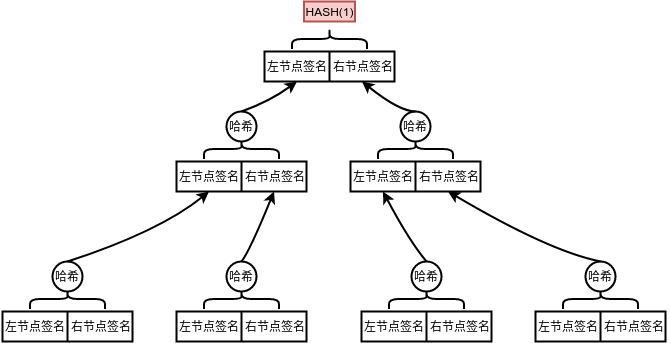
\includegraphics[scale=0.5]{Merkle-Tree.png}
    \caption{\textbf{Merkle Tree }每个节点保存着左右子树hash的签名}
   \label{fig:Merkle-Tree.png}
\end{figure}
\subsection{Merkle Tree}
为了解决上面所说的验证着需要存储大量的公钥的问题,Ralph C. Merkle提出了一种新颖的数据结构merkle tree,它能够大大的减小验证着需要保存的公钥的大小,从而减少验证者的开销。再论文中,merkle tree是用来进行前面验证,随着merkle tree
的不断发展,也被广泛的应用再完整性保护中。

如图 ~\ref{fig:Merkle-Tree.png}所示,我们以二叉树为例,在签名系统中Merkle tree中的每个节点保存着三个签名,分别是:左节点认证,右节点认证以及数据的签名。根据二叉树的组织形式,我们很容易根据父节点推到出子节点的标号,例如父节点的编号i,那么他的字节的编号分别是2i,2i+1;同理,如果我们知道子节点的编号
我们很容易知道它的父节点的编号,这一点不论在签名系统还是完整性保护系统中都显得非常的重要。因为验证者可以提前知道每一个节点以及其父子节点的编号,而不需要通过获取父节点之后才能够计算出其子节点的编号。对于一个节点中的,左右子节点认证以及消息签名,分别由三组私钥x,公钥y
完成签名认证。同时我们选择一个合适散列函数,对该节点中的公钥进行哈希计算,得到的哈希值由其对应的父节点进行签名认证。通过这样的机制,可以大大减少验证者需要知道的信息的大小。在merkle tree的验证中,验证者们只需要知道根节点的哈希值,当验证者需要验证第i条消息是否被签名者
签名过,签名者需要讲第i个消息,以及对应的公钥发给验证者。然后签名者通过自己的私钥,对需要签名的消息进行签名,并且把签名后的结果发给验证者。验证者通过公钥验证签名结果是否正确,如果通过验证,验证者将该节点所有的公钥的哈希值以及对应的父节点公钥发给用户,验证者可以通过父节点中的
公钥验证哈希值是否正确。如果当前的节点已经是根节点,因为根节点的哈希值被所有的验证者保存,验证者通过将计算得到的根节点哈希值和自己保存的根节点哈希值做对比,如果两者一致,那么整个签名的过程得到验证;反之,签名验证失败。通过merkle tree的组织形式,验证者所需要知道的共识仅限于根节点的哈希值
,另外在验证过程中,签名者会向验证者发送仅仅对数于总消息数量的信息,用于辅助验证签名的合法性。

merkle tree最初使用在签名的系统中,但是之后被广泛的应用在了完整性保护中,和签名系统中的结构相似,一、需要保护数据的完整性;二、需要保证验证者只需存储少量的信息。在完整性保护架构中,保护的数据被分成不同的数据块,采用merkle tree保护所有数据块的完整性。在数的叶子节点中,存储着所有的数据块的
哈希值,而父节点中存储着所有子节点的哈希和得哈希。数据块得完整性由叶子节点的哈希值保证,所有叶子节点哈希值得完整性由父节点保证,一次类推,我们只要保证根节点得哈希不被篡改,即可以保证数据块中数据得完整性。以merkle tree得形式保证数据得完整性,由一下几点好处:
\begin{itemize}
    \item 需要存储得可信数据很小:根节点哈希,其余节点可以存在不可信的存储中
    \item 可以并发进行数据哈希校验,每个数据块的哈希不依赖其他数据块,可以同时进行
    \item 支持数据更新后,只需要更新对应部分的哈希值即可,不需要对所有的数据进行重计算
    \item 对单个数据块完整性验证的次数和数据块的总数成对数相光
\end{itemize}
除了merkle tree的结构,还存在链表等结构,但是相较于merkle tree而言,无法并发进行完整性保护验证,以及不支持动态更新,在这里就不做更多的阐述。

\section{Bonsai Merkle Tree}
Bonsai Merkle Tree \cite{rogers2007using}在Merkle Tree上做了进一步的优化,Bonsai Merkle Tree 保留了Merkle Tree中的树状组织结构,继承了Merkle Tree中只需要保存少量的根节点哈希,能够针对少量的更新快速的重新计算哈希等等优势。但是Merkle Tree还是存在一些较为严重的问题,例如
树节点的扇出较少,无法和内存加密保护结合。因此在AISE中提出了新的完整新保护的数据结构Bonsai Merkle Tree,不同于hash tree, Bonsai Merkle Tree是以计数为基础的counter tree。hash tree节点中保存的是子节点的hash值,hash虽然能够保证数据的完整性,但是hash的大小会有严格的限制,
因为hash大小决定了哈希碰撞的概率,从而限制了一个树节的扇出。树节点的扇出较少在少量的信息保护的场景或者不关心检查开销的程序来说适用,但是在内存完整性保护上,程序非常关心实时的检查开销,树节点的扇出较少会导致树的层数较深,实时完整性检查的开销也会随之增加。一个简单的想法
是增加树的扇出,减少树节点中哈希的大小, 因此在BMT中提出了基于计数的counter tree。

\subsection{内存计数}
内存计数:counter是内存加密与完整性保护中的一个重要的概念,counter增加了内存时空维区分,来防止重放映等攻击。counter首先被使用在内存加密中,用于生成和时空相关的加密pad,之后又于完整性保护整合,作为保护对象的版本。

\textbf{基于计数的内存加密}
内存加密是内存保护中重要部分,传统的内存加密使用复杂的内存算法,会带了较为严重的运行时开销,因此在AISE中提出了一种基于counter的一次性内存加密。基于counter加密能够充分利用给时空因子,从而使一次性加密成为了可能。如图~\ref{fig:encrypt.png}所示,在AISE中,作者使用了AES算法作为加密引擎,AES算法是一种高效的加密算法,只需要经过十轮
矩阵的异或运算就能够得到相应的密文。然后单纯只是用加密算法是不够的,因为如果使用相同的key和相同的明文,得到的密文是一致的。在内存加密中,攻击者可以同时知道密文与明文,因为密文与明文之际俺的关系不会发生变化,所以攻击者可以建立起明文与密文你的对应表,从而获取内存中的数据。因此在AISE中作者没有简单的将
明文用AES进行加密,而是使用AES生成加密的pad。用pad与明文做异或的操作,从而得到密文;而解密的过程也是一致的,因为异或操作具有交换律,所以我们对密文做异或,就能够得到相应的密文,特别的异或操作往往只需要一个cycle就能够完成,并不会增加加密的开销(相较于AES加密,虽然AES已经是一个高效的加密算法了)。使用pad
对明文的数据进行加密是一个高效的加密方式,但是只能进行一次加密,因为如果攻击者同时知道明文和密文,就能够推断出加密用的pad,从何用pad对其他的数据进行加解幂。所以我们需要保证pad尽量只能使用一次。为了解决这个问题,我们为pad的生产加入相应的时空因素,其中我们使用counter来表示pad的时间因素,用访问内存地址来表示pad
的空间因素,对于相同地址的内存的每一次访问,都会是counter加一,从而保证了不可能出现两个时空因子都相同的pad。pad是由AES加密引擎生成的,通过AESk密钥,对由counter和addr拼接而成的128位seed进行加密,生成加密的pad,通过pad对明文进行异或得到对应的密文。

计数(counter)在内存加密中保证了加密pad具有一定的时空因素,也正是因为具有时空因素,所以可以使用一次性加密。在完整性保护中,完整性保护引擎巧妙地复用了counter,将counter作为完整性保护中改的版本信息,从而防止重映射等攻击。在Merkle Tree中我们主要介绍了对消息的完整性保护机制,但是没有结合内存的相关知识,这里我们将以BMT
为例,对如何保护内存的完整性,做进一步的阐述。
\begin{figure}[!htp]
    \centering
    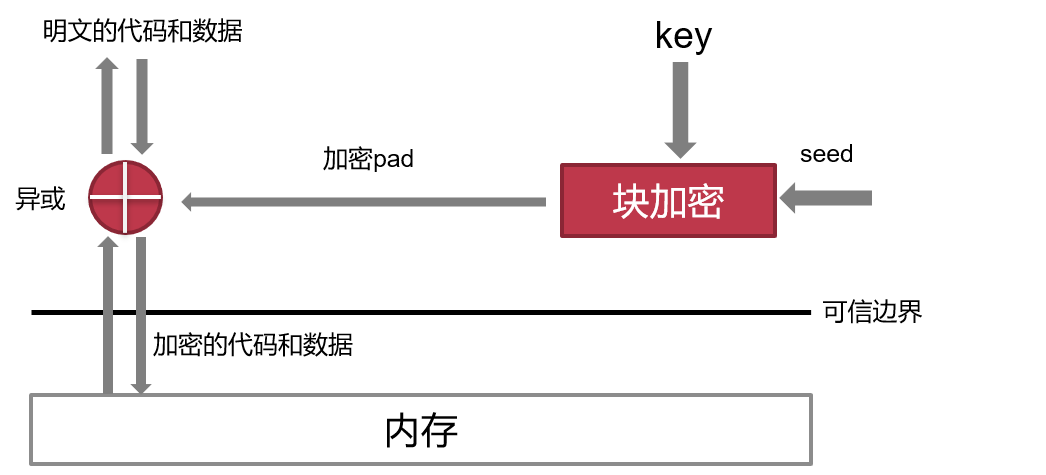
\includegraphics[scale=0.7]{encrypt.png}
    \caption{\textbf{基于计数的内存加密 }}
   \label{fig:encrypt.png}
\end{figure}

\subsection{针对内存的完整性保护}
Merkle Tree提供了一种巧妙地数据结构,通过树地形式保护消息地完整性。正如在之前章节所说地,Mekrle Tree的一大优势就是需要保护的可信数据非常少,只需要保护根节点中数据就可以了。在内存完整性保护中,内存被认为是不可信的,只有保存在SoC中的数据才是安全的(攻击的难度较大)。因为SoC中的空间大小有限,能够保存的可信数据远少于内存
中的数据。Merkle Tree的巧妙的数据结构恰好能够解决SoC中空间有限的问题,因为只需要保护根节点中的数据。

\textbf{内存攻击模型}
针对内存完整性的攻击主要分为三类:欺骗(spoofing),拼接(splicing)以及重放映(replay)。内存欺骗是指攻击者可以伪造内存中的数据,替换内存中现有的数据;内存拼接是指将其他地方的内存数据移动到受攻击的内存位置中;内存重放映是指将相同的内存地址上的老版本的数据重新写入该内存中。其中前两类攻击可以通过计算hash(HMAC)来防御。
因为攻击者无法获得hash算法的key,即无法通过已知的输入(counter,addr,明文)生成对应的合法的密文。又因为内存欺骗,和内存拼接会改变内存数据或者内存地址,导致输入三元组(明文,counter,addr)至少有一个发生了变化,所以新的输入三元组是从未出现过的,自然对应的密文也无法被攻击者直接获取。使用hash算法(HMAC)可以很好的保证
内存的欺骗,以及内存的拼接攻击,但是无法抵御内存重放的攻击。内存重放是指将同一个内存地址上的旧的数据重新加载到该内存中,在内存重放的攻击中输入三元组(counter,addr,明文)在过去曾经出现过,所以对应的密文攻击者也可以获取。攻击着可以将内存中的数据替换成为老版本的数据,来实现rollback的攻击。为了防御这类攻击,我们将Merkle Tree
中的根节点放在SoC中,在SoC中的根节点处在攻击范围之外是可信基础,所以一旦采用重放攻击,需要替换对应物理内存中所有的counter,其中包括了根节点的counter,因此攻击者无法完整重放攻击。自此,结合Merkle Tree的内存完整性保护能够很好的保护物理内存免受拼接,欺骗以及重放的攻击,结合SoC上保护的根数据,能够实现对内存的完整性保护。

\subsection{BMT数据结构}
正如之前所说的Merkle Tree存在节点的扇出较少,树的深度较深从而导致无论是运行是的开销还是内存的开销都较大(运行时开销是因为树的深度较深,检查的次数较多;内存开销较大是因为树的扇出较小,单个hash保护的数据大小是固定的,当数据规模较大时候,存储hash的开销也会随之增加)。在BMT中结合内存加密,设计了新的数据结构,希望缓解不论是运行
时候的开销还是内存开销。研究人员发现:

\begin{enumerate}
    \item Merkle Tree的设计是为了防止重放的攻击,其他的类似于内存拼接与内存欺骗可以通过计算hash对到对应数据块的MAC来防御
    \item 已有的内存加密都使用了基于counter方式,因为counter会在写内存的时候被怎家,所以也可以被当做数据块的版本号
\end{enumerate}
针对上面两个观察,研究人进一步提出,如果能够做到一下三点,那么数据不需要被Merkle Tree保护:
\begin{itemize}
    \item 所有的数据块都有自己的MAC,通过使用hash函数计算而得
    \item 计算MAC需要使用到内存块的counter和addr
    \item counter的完整性得到保护
\end{itemize}
\begin{figure}[!htp]
    \centering
    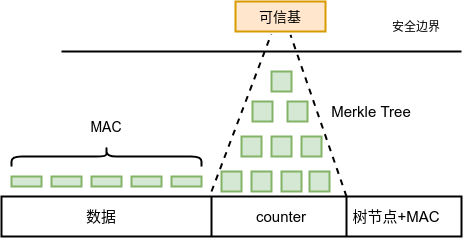
\includegraphics[scale=0.7]{counter-merkle-tree.png}
    \caption{\textbf{Bonsai Merkle Tree:}对counter的完整性保护 }
   \label{fig:counter-merkle-tree.png}
\end{figure}
如图~\ref{fig:counter-merkle-tree.png}所示,根据上述三个条件,我们发现可以通过对counter的完整性保护来代替对数据的完整性,因为counter的大小为7 bit,远小于hash的64 bit,所以对应的Merkle Tree所需要的额外内存就更少,同时因为一个cache line中可以存放更多的counter,使得树叶子节点的扇出更大,减少了树的层数,提升了运行时的性能。虽然保护counter能够比保护数据来的更有优势,但是我们
还需要论证仅仅保护counter是否能够起到和保护数据一样的安全性,下面我们将从数学的角度做严格的证明

\textbf{counter完整性保护的证明:}我们用\emph{P}和\emph{C}来表示数据块的明文与密文,数据块对应的counter用\emph{ctr}表示,对应的MAC用\emph{M}表示,hash函数\emph{H}中使用的秘钥为\emph{K}。数据块的MAC,通过使用秘钥的密码学哈希函数\emph{H}对输入密文\emph{C}和counter计算得到,例如:$M = H_K(C, ctr)$。完整性验证时候会计算MAC并且
和之前已经计算的存储在内存中的MAC进行比较,如果他们之间不匹配,那么完整性验证将失败。因为counter的完整性被保证(我们之前声明过),攻击者不能够改变\emph{ctr}却不被发现。攻击者只能够将密文\emph{C}篡改成$C^{\prime}$,或者将MAC改成$M^{\prime}$。但是因为攻击者不知道哈希函数$H$的key,所以攻击着无法生成与$C^{\prime}$匹配的$M^{\prime}$
同时因为密码学哈希函数的不可逆性,也无法根据$M^{\prime}$生成与之匹配的$C^{\prime}$,所以$M^{\prime} \neq H_K(C^{\prime}, ctr)$,从而无法通过内存的完整性检查。另外攻击者也无法将$C^{\prime}$和$M^{\prime}$同时替换成之前的老版本,因为$M^{old} = H_K(C^{old}, ctr^{old})$,但是$ctr$受到完整性保护,能够保证它一定是$ctr$和不是$ctr^{old}$。因此重放攻击也会被防御。

经过上面的证明,可以得出只需要保护counter的完整性同时就能够保证内存数据的完整性,又因为一个512 bit的数据对应的counter只有7 bit,因此需要完整性保护的数据将显著的减少,对应的Merkle Tree的大小和层数也大幅度减少,从而提升了运行是检查的性能缓解了内存的开销(Merkle Tree 从需要覆盖内存数据和counter,减少为了只需要覆盖counter。

\begin{figure}[!htp]
    \centering
    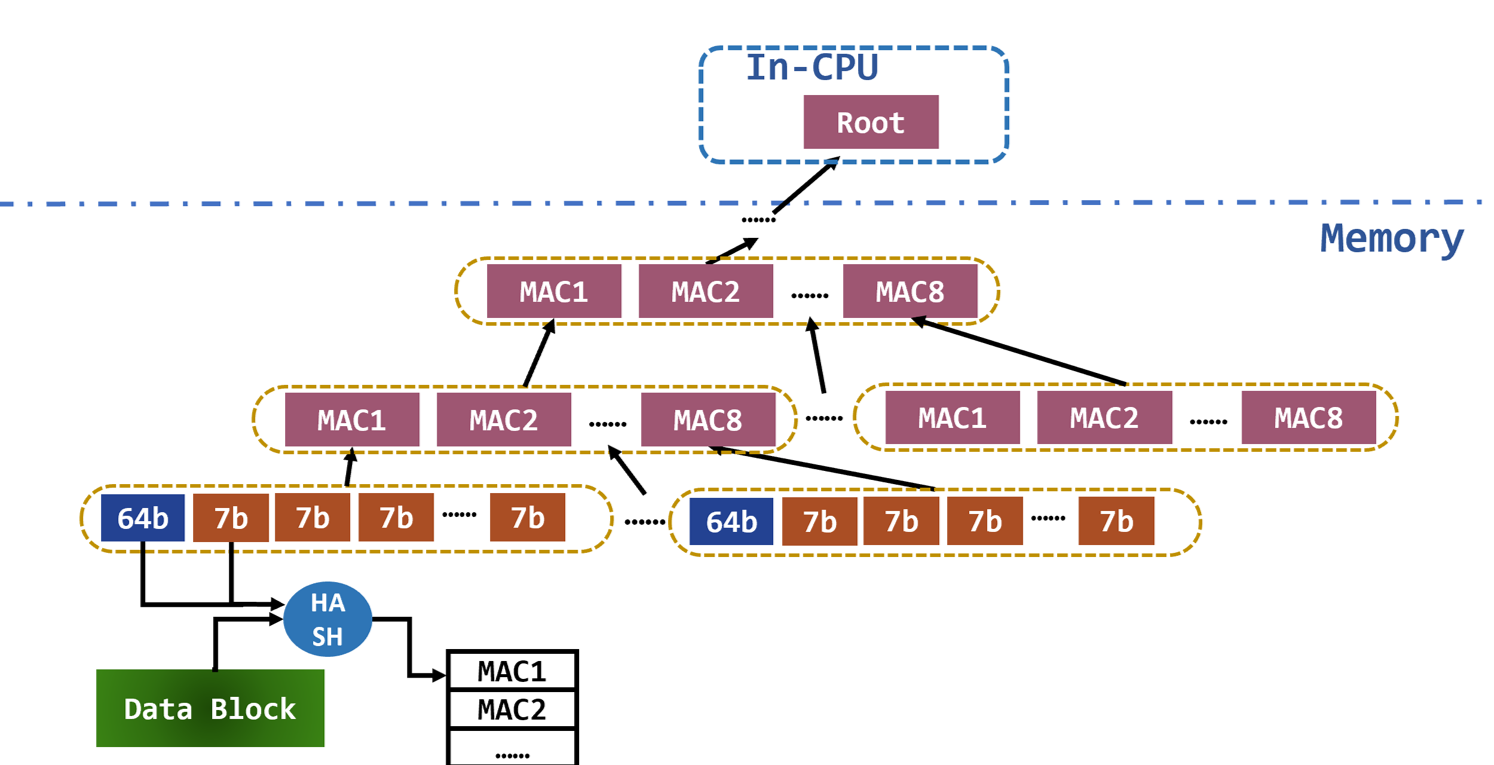
\includegraphics[scale=0.5]{BMT.png}
    \caption{\textbf{Bonsai Merkle Tree }叶子节点中保存了64个7 bit的counter}
   \label{fig:BMT.png}
\end{figure}
如图~\ref{fig:BMT.png}所示,BMT叶子节点中存储了64个7 bit的counter,每一个counter对应一个数据块。通过密码学hash函数,将counter和数据块内容进行计算生成MAC,与存储在内存中的MAC进行匹配。为了保护counter的完整性,BMT在counter上建立Merkle Tree来保证所有的counter无法被攻击者修改。每一个hash为64bit,一个树节点中能够存放8个hash,因此Merkle Tree的扇出为8。

\section{VAULT}
在BMT中,研究者发现结合基于counter的内存加密,完整性保护时只需要保护内存的counter而不需要保护内存数据本身,从而减少了Merkle Tree的内存及运行时的开销。但是BMT对完整性的保护还是基于Merkle Tree的形式。所以并没有改变Merkle Tree本身的数据结构,对于counter的保护可以理解成只增加叶子节点的扇出(从Merkle Tree扇出8增加到了64)。然后只增加叶子节点的扇出
显然是不够的,当需要保护的内存到达GB级别,叶子节点的扇出并不能起到明显的优化效果,所以我们需要尽可能的增加树中每一层的扇出。因此研究者在BMT的基础上做了进一步的拓展与优化,从而实现了对GB级别的内存完整性保护。

\subsection{全局计数与本地计数}
在BMT中采用了对counter的完整性保护,被认为是一直高效的完整性保护方式,但是不幸的是,在BMT没有在树的每一层节点中都使用counter,而只在叶子节点中将hash替换成了counter。因此在VAULT中做了一次大胆的尝试,能不能将树中每一层节点中的hash都替换成counter,这样能够提高非叶子节点的扇出。然后考虑到完整性保护树的结构特性,越在顶部的树节点越容易被访问到,所以counter
增加的也越快,出现overflow的频率也越高。我们回顾一下在BMT中使用的counter的大小位7bit,因此对统一内存写$2^7$之后就会将counter全部耗尽。counter的耗尽意味着攻击者有概率发起重放攻击,攻击者可以将内存改写成为$2^7$个版本之前的数据(因为$2^7$个版本前的内数据和当下的数据拥有相同的版本号),更少的counter bit意味着带来更大的安全风险,所以该如何兼顾安全与性能呢?
在VAULT给出了一种可行的解决办法。在VAULT的树节点中,存储着两类的counter:(a)全局的counter;(b)本地的counter,所以一个完整的counter是由一个共享的全局counter加自己都独有的本地counter。在一个树节点中(512 bit),存在一个共享的全局counter(64 bit),一个树节点hash值(64 bit)以及N个本地的counter($N*n bit$)。这样设计的好处是全局的counter解决了counter overflow的问题,因为全局的counter足够大(64 bit),如果要将全局的counter耗尽需要做$2^64$次写操作,这个在一台机器的生命周期中
基本不可能实现;而本地counter决定着树节点的扇出,相较于全局的counter,本地counter只拥有少量的bit数(在叶子节点中只有6 bit,可以存放64个本地counter),本地counter的数量决定了树节点的扇出,高扇出能够降低树的深度,减少运行时完整性检查的开销。另外考虑到树本身数据结构的特点,越往上的树节点越容易被访问到,在VAULT中不同层的树节点中本地counter的大小和个数并不相同。例如在最底层(叶子节点)中
本地counter的大小位6 bit个数位64个,而在倒数第二层中本地counter的大小12 bit个数位32。本地counter的大小不需要一直增大,因为越往上的counter越容易被CPU的cache缓存住,被cache缓存的counter被认为是安全的,当发生一次写操作的时候可以不需要增加counter的值,从而缓解较高的counter增加过快的问题。在VAULT中本地counter最大为24 bit,个数为16,因此在VAULT中树节点最小的扇出
是16,相较于Merkle Tree的扇出8来说有了一倍的提升。当保护的内存较小的时候,底层树节点的扇出更大,对性能的提升也更加的明显。

\begin{figure}[!htp]
    \centering
    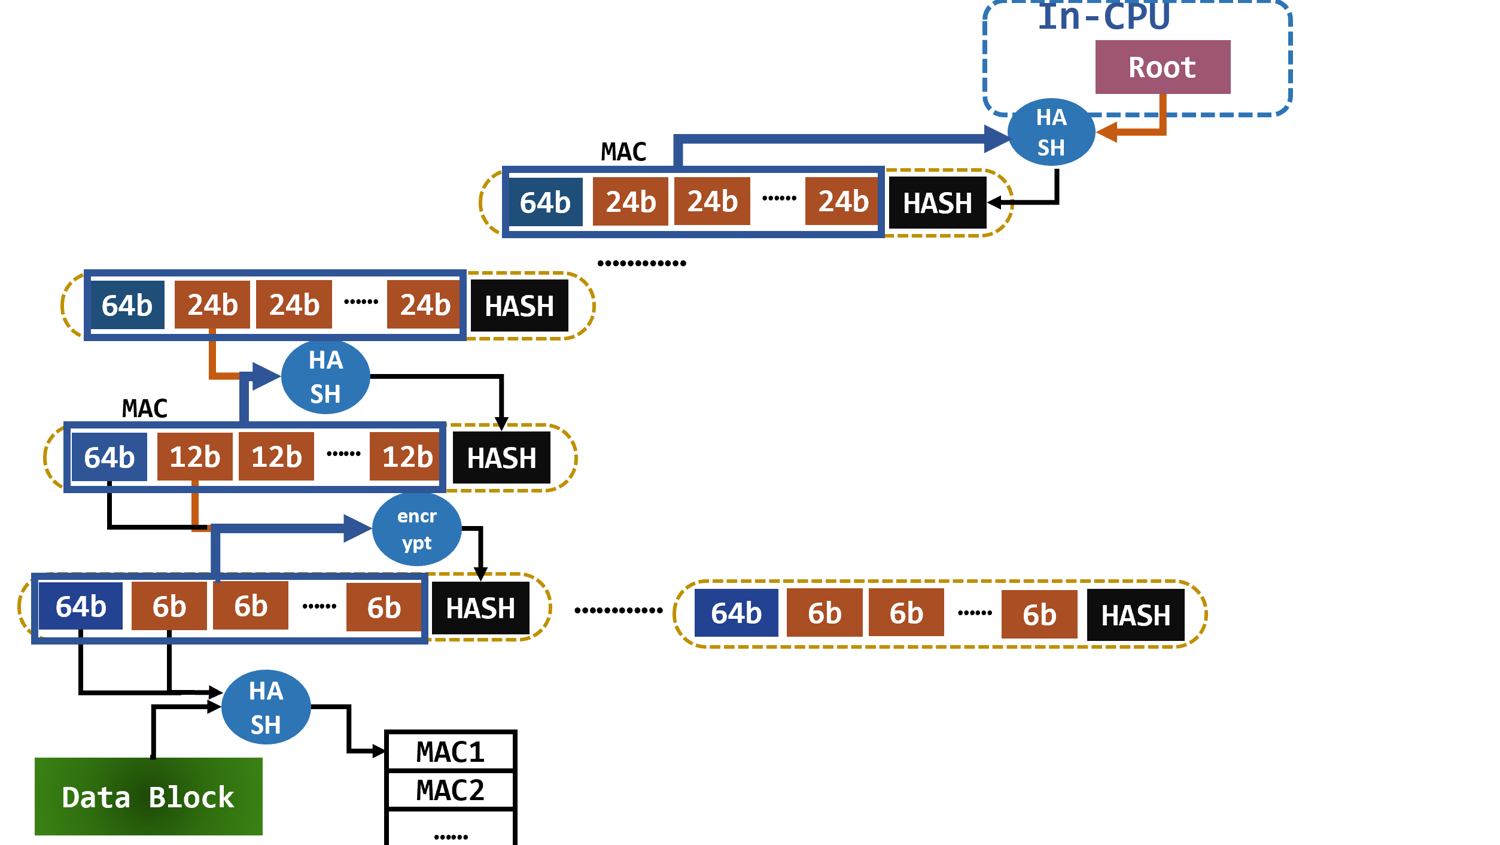
\includegraphics[scale=0.5]{VAULT.png}
    \caption{\textbf{VAULT }用counter替换hash,树节点的扇出分别为64, 32, 16}
   \label{fig: VAULT.png}
\end{figure}
\subsection{基于counter的完整性检查}
如图~\ref{fig: VAULT.png}所示,在VAULT中每一层树节点的扇出分别是:64,32,16,...,因为现在完整性保护树存储的counter和不是hash,所以应该如何保护counter的完整性呢?在上面我们提到一个树节点中除了全局的counter和本地的counter之外,还存由一个64 bit的hash,那么如何使用这个hash来保护counter的完整性呢?根据Merkle Tree的思路,所有子树的完整性由其父节点保护。在基于counter的完整性树中,将父节点中对应的counter和该节点中所有的本地counter和全局counter
分别作为hash函数的输入,计算得到相应的hash值,存储在该节点中(即64 bit的hash)。这个hash的生成包括了该节点所有counter的信息,以及父节点中对应counter的信息,只要保证父节点钟大哥counter的完整性,那么攻击者无法通过修改该节点中的counter值来生成合法的hash值,下面我们将具体介绍读操作和写操作的完整性检查与更新。

\textbf{读和验证:}当发生一次读请求时,内存控制器首先会读取内存数据,内存数据对应的MAC以及完整性保护树中的叶子节点。内存控制器会根据叶子节点中的counter以及内存数据进行哈希计算(HMAC)将计算得到的MAC值与存储的MAC做匹配,如果不匹配,那么完整性保护检查失败。之后内存控制器会去索引叶子节点对应的父节点中的counter,将父节点中的counter和叶子节点中所有的counter进行哈希计算,得到对应的MAC值,
将计算的到的MAC值与存储在叶子节点中的MAC值进行匹配,如果不一致,那么完整性保护检查失败。重复上诉步骤,直到父节点的counter处在SoC中,或者父节点即为根节点,则完整性保护检查结束,验证通过。

\textbf{写和更新:}当放生一次写请求时,内存控制器奖新数据写到对应的内存块中,然后增加完整性保护树中的叶子节点counter数值。之后内存控制器中的完整性保护引擎根据新的内存数据和增加的counter计算出新的MAC值,然后将更新后的MAC值写回到内存数据对应的MAC中。之后内存控制器会增加叶子节点对应的父节点中的counter值,同时将叶子节点中所有的counter和增加过的父节点counter进行hash计算
得到新的MAC值,将新的MAC值写入叶子节点中存放MAC的区域。重复上诉步骤,直到当前节点的counter已经在SoC中,或者父节点为根节点,则一次写操作的更新完成,同时为写入的新数据提供了完整性保护。
